\begin{frame}		
	\frametitle{Sliding Window}
	\framesubtitle{Go Back N. Principle}
		\begin{figure}[H]
			\center{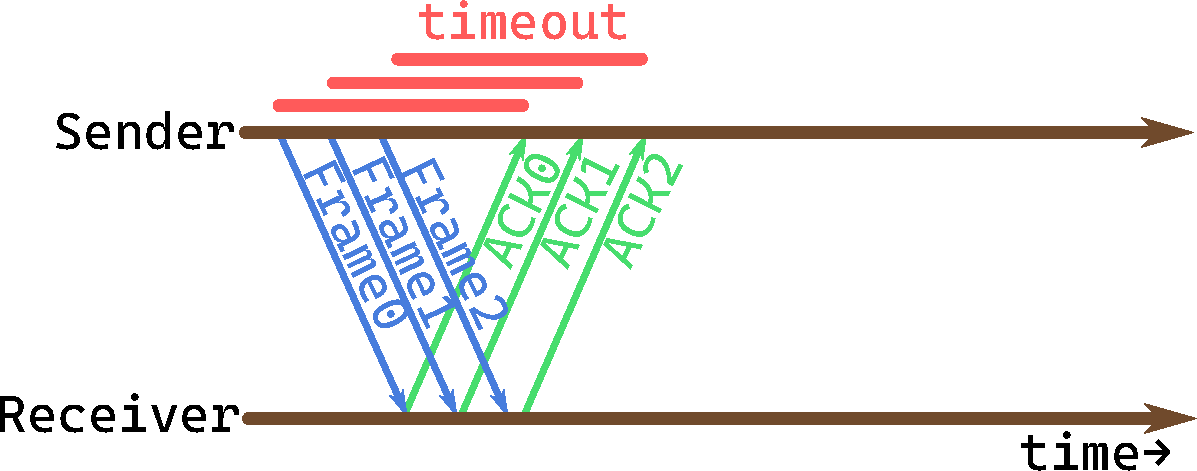
\includegraphics[width = 1\textwidth]{gbn-1}}
		\end{figure}
\end{frame}

\begin{frame}		
	\frametitle{Sliding Window}
	\framesubtitle{Go Back N. Principle}
	\begin{figure}[H]
		\center{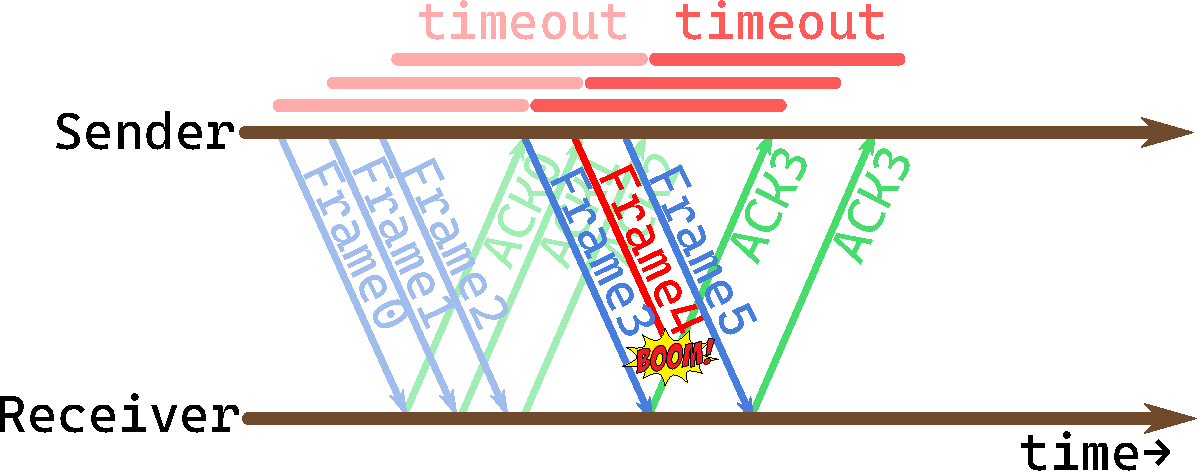
\includegraphics[width = 1\textwidth]{gbn-2}}
	\end{figure}
\end{frame}

\begin{frame}		
	\frametitle{Sliding Window}
	\framesubtitle{Go Back N. Principle}
	\begin{figure}[H]
		\center{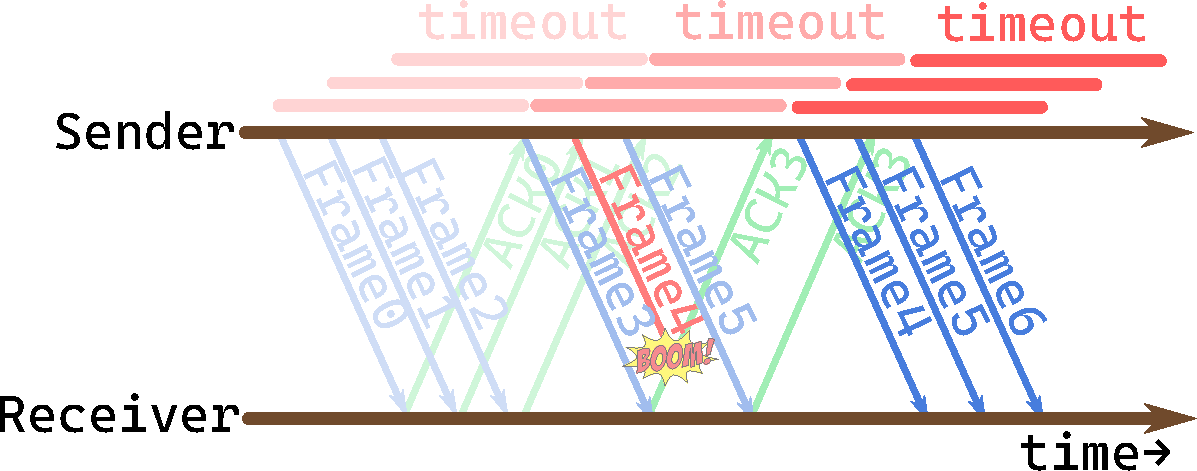
\includegraphics[width = 1\textwidth]{gbn-3}}
	\end{figure}
\end{frame}

\begin{frame}		
	\frametitle{Sliding Window}
	\framesubtitle{Efficiency of GoBack-N}
	\begin{itemize}
		\item Probability of Failure\footnotemark:
		$P_f = 1 - (1-plr)^2$
		\item Average total time to transmit a packet [\cite{1}]. Windows size $W_s$ should implies to be selected so that the channel will be busy all the time.
		$$E[t_{packet}] = t_f \dfrac{1 + (W_s - 1) P_f}{1-P_f}$$
		\item Effective information transmission rate: $R_{eff} =\dfrac{n_f - n_{headers}}{E[t_{packet}]} $
		\item Associated transmission efficiency: $\eta = \dfrac{R_{eff}}{Rate}$
		

		
	\end{itemize}
\end{frame}